% ssss.tex
本節針對四邊簡支 (SSSS) 邊界條件進行分析。邊界條件為 $w = 0$ 且彎矩 $M_n = 0$（切向轉角無約束）。解析解可由 Navier 雙重傅立葉級數獲得。

\subsection{解析解}
Mindlin 板四邊簡支的固有頻率滿足三次頻率方程：
\begin{equation}
A \omega^4 - B \omega^2 + C = 0
\end{equation}
其中
\begin{align}
A &= \rho h I_2,\quad
B = \rho h D \lambda^2 + D^s (\rho h + I_2 \lambda^2),\quad
C = D D^s \lambda^4, \\
\lambda^2 &= \left(\frac{m\pi}{a}\right)^2 + \left(\frac{n\pi}{b}\right)^2
\end{align}
取最低的兩個根中對應彎曲模態者，無因次化頻率為 $w_h = \omega a^2 \sqrt{\rho h / D}$。

\subsection{數值方法}
採用有限元素法，對彎曲項使用完全積分，剪切項使用縮減積分以避免剪切鎖死。網格收斂性以 $n_{\text{div}} = 9 \sim 25$ 進行。

\subsection{誤差定義}
定義相對誤差（對數尺度）：
\begin{equation}
\text{Error} = \log_{10} \left| \frac{w_{h,\text{FEM}} - w_{h,\text{exact}}}{w_{h,\text{exact}}} \right| \label{eq:error}
\end{equation}
$x$ 軸為網格劃分數 $n_{\text{div}}$（或特徵長度 $h$），$y$ 軸為 $\log_{10}$ 相對誤差。

\subsection{結果}
圖~\ref{fig:ssss_modes} 展示前六階模態的無因次頻率與誤差隨網格加密的變化，圖~\ref{fig:ssss_mode_shapes} 為典型的模態形狀。

\begin{figure}[H]
\centering
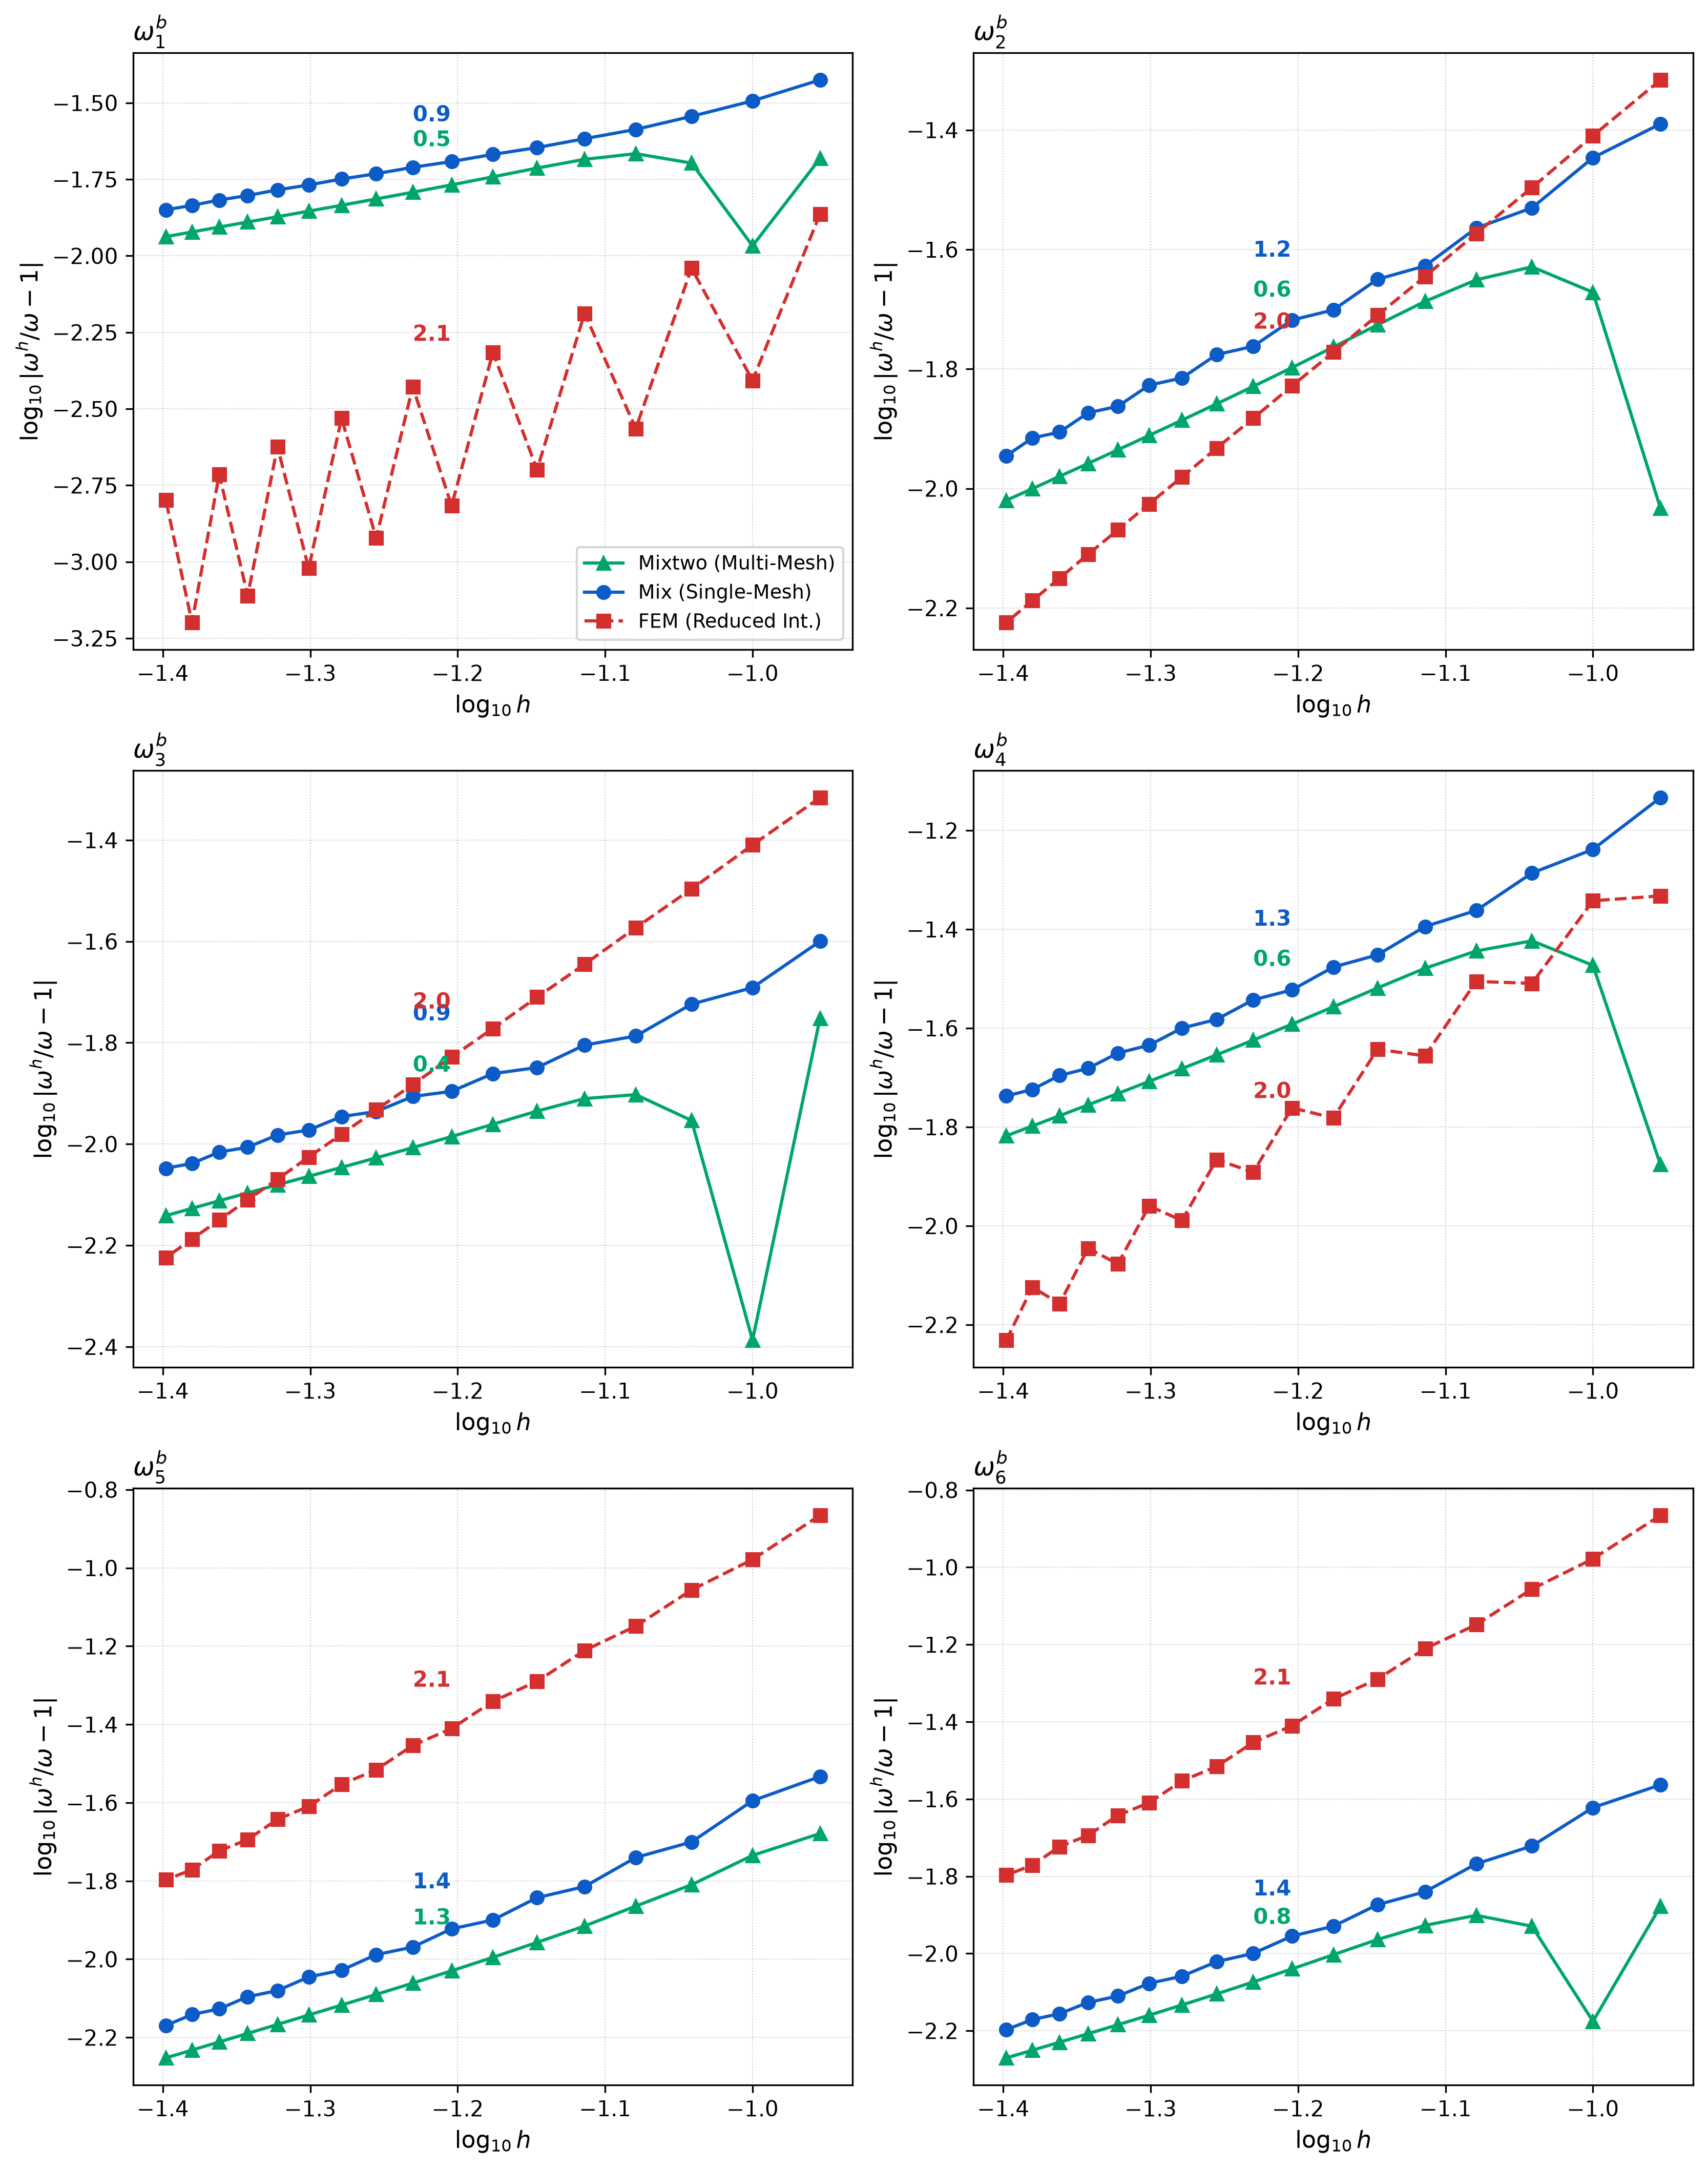
\includegraphics[width=\textwidth]{mode_6plots_4s.png}
\caption{四邊簡支 Mindlin 板前六階模態收斂圖。上排：無因次頻率 $w_h$；下排：$\log_{10}$ 相對誤差。}
\label{fig:ssss_modes}
\end{figure}

觀察結果可知，隨著網格加密，所有模態的頻率均單調收斂，且誤差呈線性下降，驗證方法之有效性。

